\documentclass{article}

%Aus dem LaTex Template der Universit�t Stuttgart
%------------------------------------------------
\usepackage[utf8]{inputenc}
\usepackage[T1]{fontenc}
\usepackage[sfdefault]{ClearSans} %% option 'sfdefault' activates Clear Sans as the default text font
\usepackage{cmap}
\usepackage[ngerman]{babel}
\usepackage{graphicx}
\usepackage[pdftex,hyperref,dvipsnames]{xcolor}
\usepackage{listings}
\usepackage[a4paper,lmargin={2cm},rmargin={2cm},tmargin={3.5cm},bmargin = {2.5cm},headheight = {4cm}]{geometry}
\usepackage{amsmath,amssymb,amstext,amsthm}
\usepackage[lined,algonl,boxed]{algorithm2e}
\usepackage{tikz}
\usepackage{hyperref}
\usepackage{url}
\usepackage[inline]{enumitem} % Erm�glicht �ndern der enum Item Zahlen
\usepackage[headsepline]{scrpage2} 
\usepackage{algorithmic} % F�r Pseudocode
\usepackage{ marvosym } % f�r Pfeil(e)
\usepackage{booktabs} % F�r die sch�neren Booktabs-Tabellen
\usepackage{tikz}
\usepackage{pdfpages}
\usepackage{blindtext}
\usepackage{scrextend}
\usepackage{pdfpages}
\usepackage{natbib} % Yannis hat das importiert; TODO: nachfragen, zu was das gut ist
\pagestyle{scrheadings} 
\usetikzlibrary{automata,positioning}

\begin{document}
	%%% Vorgegebenes Deckblatt %%%
	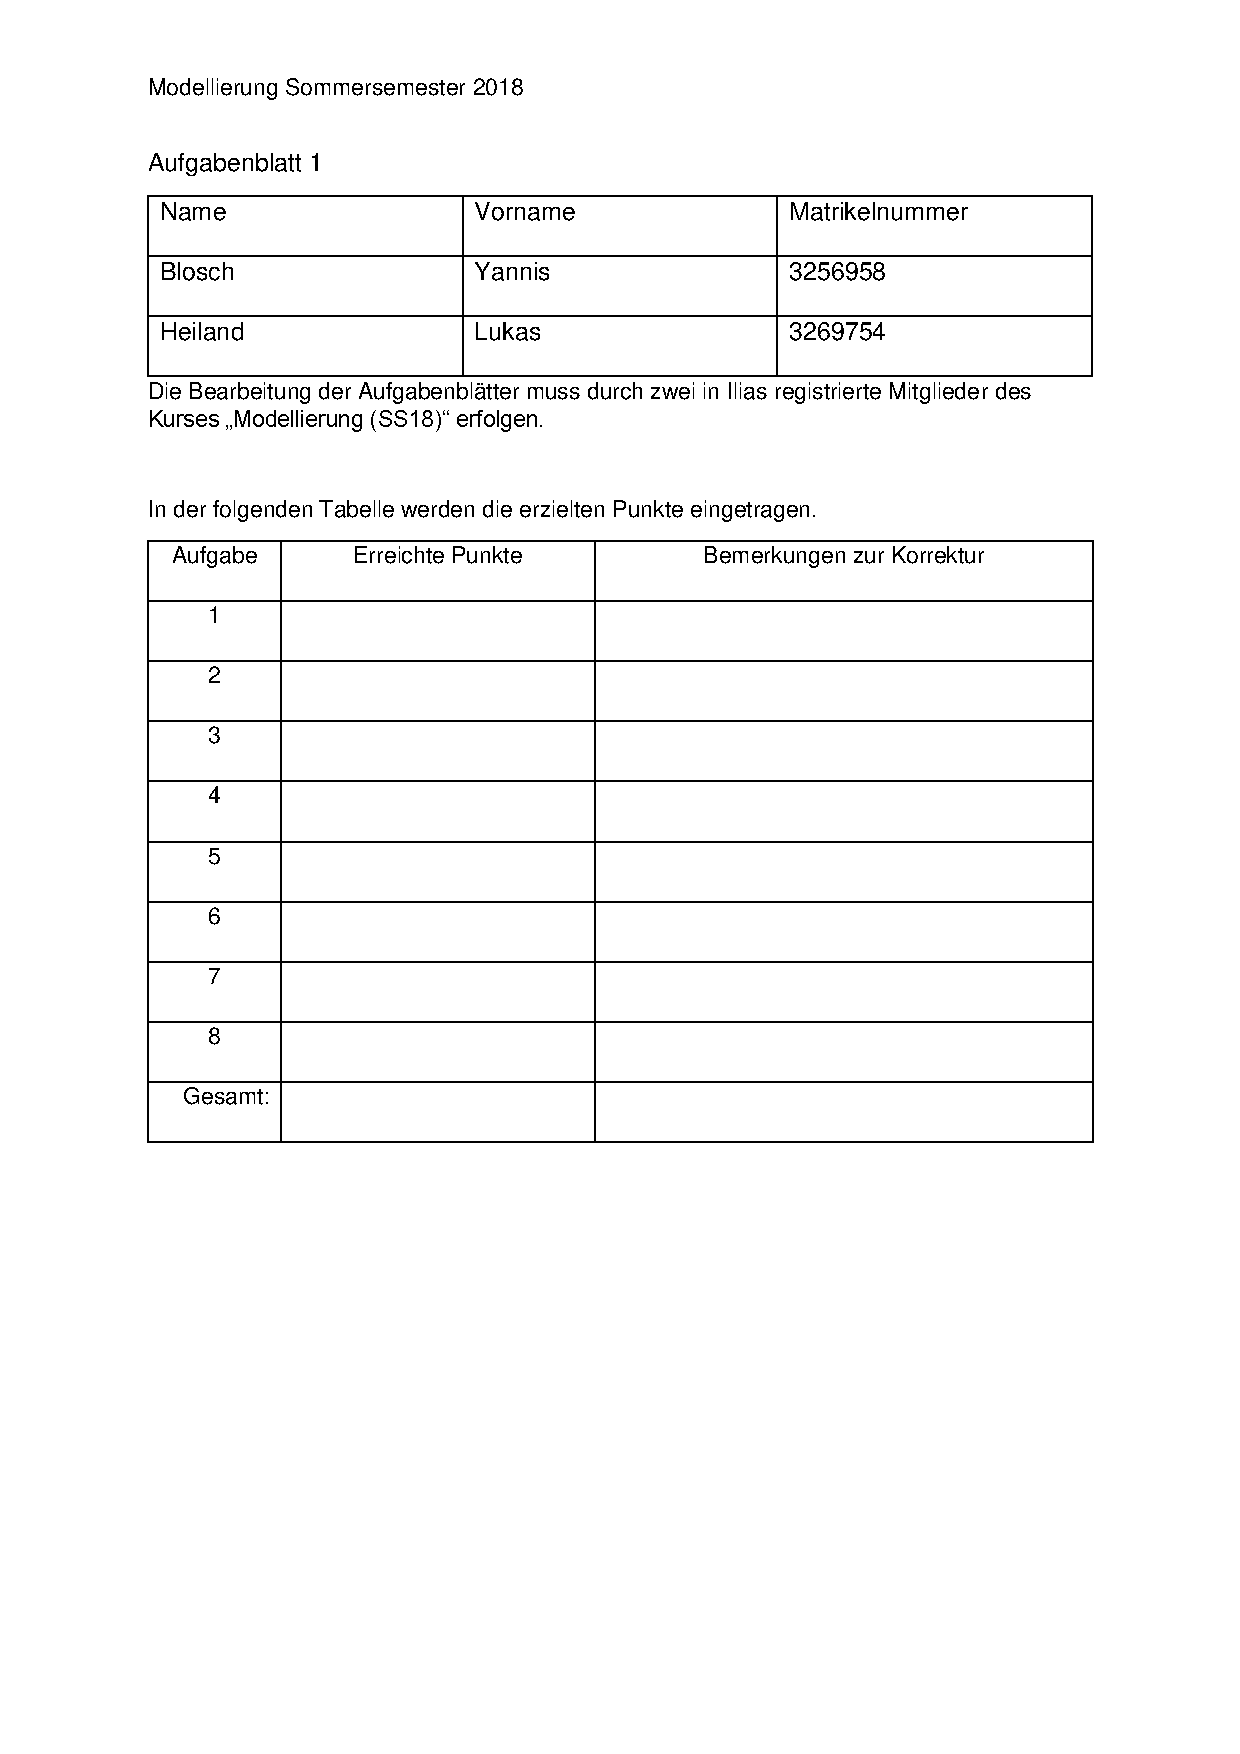
\includepdf{deckblatt.pdf}
	%%% format and header %%%
	% Counter für das Blatt und die Aufgabennummer.
% Ersetze die Nummer des Übungsblattes und die Nummer der Aufgabe
% den Anforderungen entsprechend.
% Beachte:
% \setcounter{countername}{number}: Legt den Wert des Counters fest
% \stepcounter{countername}: Erhöht den Wert des Counters um 1.
\newcounter{sheetnr}
\setcounter{sheetnr}{1} % Nummer des Übungsblattes
\newcounter{exnum}
\setcounter{exnum}{1} % Nummer der Aufgabe

% Befehl für die Aufgabentitel
\newcommand{\exercise}[1]{\section*{Aufgabe \theexnum\stepcounter{exnum} #1}} % Befehl für Aufgabentitel

% Formatierung der Kopfzeile
% \ohead: Setzt rechten Teil der Kopfzeile mit
% Namen und Matrikelnummern aller Bearbeiter
\ohead{Yannis Blosch (3256958)\\
Lukas Heiland (3269754)}
% \chead{} kann mittleren Kopfzeilen Teil sezten
% \ihead: Setzt linken Teil der Kopfzeile mit
% Modulnamen, Semester und Übungsblattnummer
\ihead{Modellierung\\
Sommersemester 2018\\
Blatt \thesheetnr}
	
	\section*{Aufgabe 5.1}
		\paragraph*{a.} Ein Schl"usselkandidat $ \Gamma $ enth"alt alle Attribute, die auf keiner rechten Seite der funktionalen Abh"angigkeiten in $ \mathcal{X} $ stehen. Des Weiteren muss f"ur alle Attribute $A \in \mathcal{R} $ gelten: $ A \in (\Gamma)^+ $; dar"uber hinaus muss $ \Gamma $ minimal sein, d.h. es darf keine andere Attributmenge geben, die die vorigen Anforderungen erf"ullt und weniger Elemente enth"alt als $ \Gamma $.\\
		\textbf{Vorbemerkung:} Da nur L auf keiner rechten Seite von $ \mathcal{X} $ vorkommt, muss L in jedem candidate key vorkommen. Des Weiteren ist $ (L^+) = \{L,E,J\} \neq \mathcal{R} \Rightarrow $ jeder candidate key muss mindestens zwei Attribute enthalten.\\[1.2em] 
		%%%%%%%%%%%%%%%%%%%%%%%%%%%%%%%%%%%%%%%%
		%%%%%%%%%%%%%%%%% 1. CK %%%%%%%%%%%%%%%%
		%%%%%%%%%%%%%%%%%%%%%%%%%%%%%%%%%%%%%%%%
		\textbf{1. Schl"usselkandidat: }$ \mathbf{DL }$
		\begin{itemize}
			\item L steht auf keiner rechten Seite, $ L \in DL $ \checkmark
			\item $ (DL)^+: 0. \{D,L\} $\\
			$ 1. \{D,L,E,G,H\} $ \hspace*{20mm}wegen $ DL \rightarrow EGH $\\
			$ 2. \{D,L,E,G,H,J\} $ \hspace*{17mm}wegen $ E \rightarrow J $\\
			$ 3. \{D,L,E,G,H,J,F,K\} $ \hspace*{9mm}wegen $ G \rightarrow FK $\\
			$ \Rightarrow \mathcal{R} = (DL)^+$ \checkmark
			\item $ DL $ ist minimal (folgt aus Vorbemerkung) \checkmark\\[1.2em]
		\end{itemize}
		%%%%%%%%%%%%%%%%%%%%%%%%%%%%%%%%%%%%%%%%
		%%%%%%%%%%%%%%%%% 2. CK %%%%%%%%%%%%%%%%
		%%%%%%%%%%%%%%%%%%%%%%%%%%%%%%%%%%%%%%%%
		\textbf{2. Schl"usselkandidat: }$ \mathbf{LH} $
		\begin{itemize}
			\item L steht auf keiner rechten Seite, $ L \in LH $ \checkmark
			\item $ (LH)^+: 0. \{H,L\} $\\
			$ 1. \{H,L,D,G\} $ \hspace*{23mm}wegen $ H \rightarrow DG $\\
			$ 2. \{H,L,D,G,E\} $ \hspace*{19mm}wegen $ L \rightarrow E $\\
			$ 3. \{H,L,D,G,E,F,K\} $ \hspace*{10mm}wegen $ G \rightarrow FK $\\
			$ 4. \{H,L,D,G,E,F,K,J\} $ \hspace*{7mm}wegen $ E \rightarrow J $\\
			$ \Rightarrow \mathcal{R} = (LH)^+ $ \checkmark
			\item $ LH $ ist minimal (folgt aus Vorbemerkung) \checkmark
		\end{itemize}	
	
	%%% b) DL -> EGH enthält L -> E
	%%% DLEGH bleiben, FJK in neue Tabelle mit E als foreign key und neue Tabelle mit DLEF
		\paragraph*{b.}\textbf{1. Schl"usselkandidat}\\
		E und J sind partiell abh"angig vom candidate key, n"amlich von L. Schema in 2NF:\\
		$ \mathcal{R}_1(\underline{D},F,G,H,K,\underline{L}) $, $ \mathcal{R}_2(\underline{L},E,J) $\\[1.2em]
		
		\textbf{2. Schl"usselkandidat}\\
		D, G,F, und K sind nur von H abhängig, also partiell vom candidate key. Schema in 2NF:\\
		$ \mathcal{R}_1(D,F,G,\underline{H},K) $, $ \mathcal{R}_2(E,J,\underline{L}) $, $ \mathcal{R}_3(\underline{H},\underline{L}) $
		
	%%% c) eigentlich kann man den 2. Teil von a) kopieren
		\paragraph*{c.}$ CLOSURE(\{L,H\}, \mathcal{X}):$\\
		$ 0. \{H,L\} $\\
		$ 1. \{H,L,D,G\} $ \hspace*{25mm}wegen $ H \rightarrow DG $\\
		$ 2. \{H,L,D,G,E\} $ \hspace*{21mm}wegen $ L \rightarrow E $\\
		$ 3. \{H,L,D,G,E,F,K\} $ \hspace*{13mm}wegen $ G \rightarrow FK $\\
		$ 4. \{H,L,D,G,E,F,K,J\} $ \hspace*{9mm}wegen $ E \rightarrow J $\\
		$ \Rightarrow F \in CLOSURE(\{L,H\}, \mathcal{X}) \rightarrow$ \checkmark
	\pagebreak
	%%% d) LH -> H, H -> DG, DG-> G, G-> FK, FK -> F
		\paragraph*{d}.\\
		1. $ LH \rightarrow H $ \hspace*{40mm}reflexivity ($ H \subseteq LH $)\\
		2. $ LH \rightarrow DG $ \hspace*{37mm}transitivity mit 1. und $ H \rightarrow DG $\\
		3. $ DG \rightarrow G $ \hspace*{40mm}reflexivity ($ G \subseteq DG $)\\
		4. $ LH \rightarrow G $ \hspace*{40mm}transitivity mit 2. und 3.\\
		5. $ LH \rightarrow FK $ \hspace*{37mm}transitivity mit 4. und $ G \rightarrow FK $\\
		6. $ FK \rightarrow F $ \hspace*{40mm}reflexivity ($ F \subseteq FK $)\\
		7. $ LH \rightarrow F $ \hspace*{40mm}transitivity mit 5. und 6.\\
	
	
	%%%%% 5.2
	\section*{Aufgabe 5.2}
	\paragraph*{1.NF gegeben, alle Werte atomar}
	\paragraph*{2.NF gegeben, keine partielle Abh"angigkeit vorhanden}
	\paragraph*{3.NF gegeben, keine transitiven Abh"angigkeiten}
	\paragraph*{BCNF:}
	C ist eine Determinante (B ist voll funktional abh"angig von C), gehört aber nicht zum candidate key ($ \mathcal{R} $ in BCNF $ \Leftrightarrow $ Jede Determinante muss ein candidate key sein) $ \Rightarrow \mathcal{R} $ nicht in BCNF. Schema in BCNF:\\
	$ \mathcal{R}_1(\underline{A,C}) $, $ \mathcal{R}_2(B,\underline{C}) $
	
	
	%%%%% 5.4 a) BH
	
	\section*{Aufgabe 5.4}
		\paragraph*{a.}Ein Schl"usselkandidat $ \Gamma $ enth"alt alle Attribute, die auf keiner rechten Seite der funktionalen Abh"angigkeiten in $ \mathcal{X} $ stehen. Des Weiteren muss f"ur alle Attribute $A \in \mathcal{R} $ gelten: $ A \in (\Gamma)^+ $; dar"uber hinaus muss $ \Gamma $ minimal sein, d.h. es darf keine andere Attributmenge geben, die die vorigen Anforderungen erf"ullt und weniger Elemente enth"alt als $ \Gamma $. \\[1.1em]
		
		
		
		%%%%% 5.4 b) BH -> AC, A -> F bzw AC -> F
		\paragraph*{b.} D ist partiell abh"angig von BH, denn $ B \rightarrow D $ 
		
		
		\paragraph*{c.}Es gibt eine transitive Abhängigkeit vom candidate key: $ DE \rightarrow A \rightarrow B $
		
		
		\paragraph*{d.}$ \mathcal{S} $ ist nicht in 3NF, da es eine transitive Ab"angigkeit gibt: $ DE \rightarrow A \rightarrow B $
\end{document}